\section{Training a Neural Network for Speech Recognition}\label{ds}
As stated above, the title of this thesis may be a bit misleading because the focus for this project is not on training a state of the art \ac{STT} engine. This chapter describes the reference model, the simplified model and how they were compared.

\subsection{\textit{DeepSpeech}: A reference model}

A \ac{NN} that had quite an impact on \ac{ASR} was \textit{DeepSpeech} \parencite{deepspeech}. It reached recognition rates near-par to human performance, despite using a comparably simpler than traditional speech systems. Because the relation between audio signal and text was learned \ac{E2E} the network was also pretty robust to distortions like background noise or speaker variation. An open source implementation of  \textit{DeepSpeech} is available from Mozilla \footnote{\url{https://github.com/mozilla/DeepSpeech}}. This implementation was written in C and Python and uses the \textit{TensorFlow} framework. Although sticking to the architecture proposed by \cite{deepspeech}, it represents a variant of of the model proposed in the paper \parencite{ctc_paper}, because it uses \ac{MFCC} as features whereas the original paper proposes raw spectrograms. Since the implementation also uses a \ac{LM}, the quality of the model is measured as the percentage of misspelled or wrong words (referred to as \ac{WER}) or as the edit distance (also called Levenshtein distance or \ac{LER}). A pre-trained model for inference of English transcript can be downloaded, which achieves a \ac{WER} of just 6.5\%, which is close to what a human is able to recognize \parencite{mozillajourney}. \textit{DeepSpeech} serves as a reference model for the simplified model used in this project.

\subsection{Related research}

The idea of training a \ac{STT} model on limited data has also been researched by \cite{budget}, although with a different approach. Instead of training a \ac{RNN} from scratch, they used a \ac{CNN} trained to recognize English as a base. This network used the \textit{Wav2Letter} \parencite{wav2letter} architecture whose lower layers were frozen and whose higher layers were re-trained on a (smaller) German corpus, a process is also known as Transfer Learning. 

Similar to \textit{DeepSpeech}, the model trained by \cite{budget} uses a \ac{LM} to decode the model output into character sequences, \ac{CTC} as its loss function\footnote{although the original \textit{Wav2Letter} model uses an alternative loss function} and (mel-scaled) spectrograms as features. The German audio and text data used to train the higher layers were taken from several (very heterogenous) corpora from the Bavarian Archive for Speech Signals (BAS). 

\cite{budget} were lead by the assumption that languages -- especially such belonging to the same family -- share common features that can be transferred by sharing the pre-trained lower layers that detect them. This assumption was proved true, yielding a model that could be trained faster and with less training data while producing results of similar quality provided the network was trained for a certain amount of time.

Although the experiments conducted by \cite{budget} suggest an interesting starting point to train a model for the \ac{ASR} stage in this pipeline, this is not the path taken in this project for the following reasons:

\begin{itemize}
	\item The training data used by \cite{budget} is still much larger (300+ hours) than the data available from the IP8 project. Achieving the same amount of training data would require some heavy preprocessing, which according to experience eats up most of the project time. It would also mean that the efforts made in the IP8 project are discarded.
	\item Because \cite{budget} follow a completely different approach than this project, it would mean starting from scratch and neglecting the insights made in the IP8 project.
	\item Since \textit{DeepSpeech} is used as the reference model, it may make more sense comparing it to a simplified version of itself rather than a completely different model using a \ac{CNN} architecture. Because the impact of non-trivial properties like architecture is much more limited, this makes the two networks much more comparable in that different results can be attributed to the simplifications made.
\end{itemize}

For those reasons I consider the experiments made by \cite{budget} an interesting alternative. However, to leverage the efforts made in the IP8 project, the goal for this project is still to train a stripped-down version of the \textit{DeepSpeech} model rather than transfer-learning.

\subsection{Exploiting the \textit{DeepSpeech} model}

The final \ac{FA} pipeline should provide alignments for any language. One possible approach would be to train a model using the existing Mozilla implementation by providing training-, validation- and test-data for each language. However, this approach does not fullfill the premises initially made:

\begin{enumerate}
	\item The \textit{DeepSpeech} implementation was explicitly designed for \ac{ASR}. In such settings a low \ac{WER} is desirable. But because accurate speech recognition is not the main concern in this project, the architecture of the Mozilla implementation might be overly complicated.
	\item The Mozilla implementation requires an (optional) \ac{LM}, which is tightly integrated with the training process which might not be available for the target languages.
\end{enumerate}

For these reasons, a simplified version of the \textit{DeepSpeech} model was derived from the Mozilla implementation. This version should (hopefully) require less training data to converge and still produce partial transcriptions that can be aligned.

\subsection{A simpler model}

The model from the IP8 project had some serious performance issues and did also not produce transcripts that were even remotely recognizeable as human language. It was therefore not usable and is further referred to as \textit{previous model}. In the course of this project, it was examined more closely to find out what works best and to help the model converge. A few changes were made to arrive at a new model which was able to learn something meaningful. This model is further referred to as \textit{new model}. The new model started to infer transcripts that -- although far from perfect -- resembled the ground truth. 

\subsubsection{Differences between the IP8- and the IP9-model}
The following list summarizes the differences between the previous and the new model:

\begin{itemize}
	\item \textbf{Optimizer}: The new model uses \ac{SGD}, whereas the previous model used Adam. Adam was used in the previous model because it works very well in various circumstances. It is also the Optimizer used in the Mozilla implementation of \ac{DS}. This Optimizer prevents getting stuck at local optima or saddle points by computing adaptive learning rates. It does so by keeping a history of exponentially decaying average of past gradients. However, this optimizer did not seem to work for the simplified model. Despite trying out various values for the parameters, I could not find a working combination. \ac{SGD} on the other hand worked out-of-the-box with default parameter values from Keras. Because of time constraings, I decided to stick with \ac{SGD}, at the risk of missing the optimal parameters.
	\item \textbf{number of features}: The previous model used 13 \ac{MFCC} as features. This number is often found in research papers about acoustic modelling. The Mozilla implementation of \textit{DeepSpeech} however doubled this number to $26$. The new model uses the same number of features. Despite the sharp increase, this value is still much smaller than the $160$ filter banks used in the original \textit{DeepSpeech} model. The amount of training data is therefore still expected to be smaller than in the original model.
\end{itemize}

\subsubsection{Differences between the simplified and the reference model}
The new model is a simplified variant of the Mozilla implementation of the \textit{DeepSpeech} model with the following simplifications and changes applied:

\begin{itemize}
	\item \textbf{Different use of LM}: The likelihood \textit{score} of a sequence of words is calculated by an \ac{LM}. This score is tightly integrated with the training process in the Mozilla implementation, providing adjustable hyperparameters to weigh the score or the number of valid words. The simplified model also uses a \ac{LM}, but does not use such hyperparameters. In fact, the \ac{LM} is not included in the training process. Instead, the \ac{LM} is applied in some sort of post-processing to improve the quality of the inferred transcriptions a posteriori (see next chapter).
	\item \textbf{No convolution in first layer}: Whereas \cite{ctc_paper} propose a convolution over time in the first layer for performance reasons, this is not done in the simplified model.
	\item \textbf{LSTM instead of SimpleRNN}: Whereas \cite{ctc_paper} deliberately refrain from using \ac{LSTM} cells for various reasons, the Mozilla implementation has shown that it is possible to implement the \textit{DeepSpeech} model using \ac{LSTM} cells. Since the simplified model is based on the Mozilla implementation, it also uses \ac{LSTM} cells.
	\item \textbf{dynamic alphabet}: The Mozilla implementation uses an alphabet with 29 characters\footnote{${a,b,c,...,z, space, apostrophe, blank}$}, which is also what is proposed in the \textit{DeepSpeech} paper. This is due to the fact that apostrophes are frequently found in English word tokens (like \textit{"don't"} or \textit{"isn't"}). The apostrophe is therefore an integral part of English words, but not for other languages. Vice versa, other languages may use a different alphabet (like German, where umlauts are prevalent). Because the number of characters in the alphabet determines the number of nodes in the output layer, the output layer has different shapes for different languages.
	\item \textbf{no context}: The \textit{DeepSpech} paper proposes using combining each feature vector $x_t$ (a frame in the spectrogram) with $C \in \left\{ 5,7,9 \right\}$ context frames. This context frame was dropped to keep the nuber of features in the input layer small. As a result, the first layer in the model only depends on the $26$ features of the feature vector $x_t$.
	\item \textbf{no convolution in input layer}: The \textit{DeepSpeech} paper proposes a series of optimization to reduce computational cost. Among these optimization is a convolution over time in the input layer with by striding with step size $2$. Because the context frame was dropped in this project, the striding was also not applied in order not to lose the information from the intermediate frames.
\end{itemize}


Figure \ref{model_architecture} shows the architecture proposed in the \textit{DeepSpeech} with the changes applied for this project. It looks similar to the one shown in the paper. Note the missing context frame, the use of \ac{MFCC} features and \ac{LSTM} cells in the recurrent layer.

\begin{figure}[h!]
	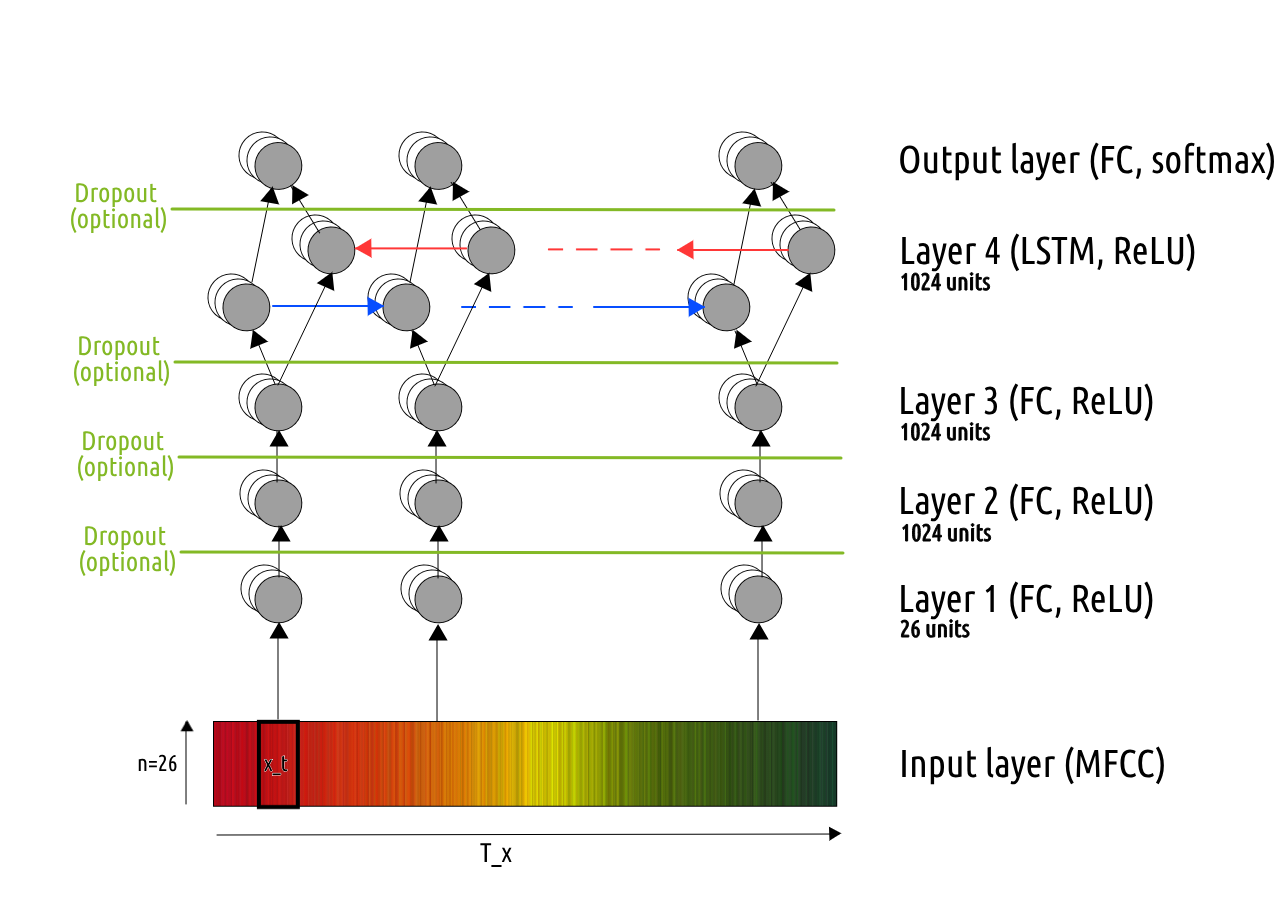
\includegraphics[width=\linewidth]{./img/model_architecture.png}
	\caption{Architecture of the simplified model. The cell type and the activation function is indicated in brackets for each layer (FC=Fully-Connected, ReLU=Rectified Linear Unit)}
	\label{model_architecture}
\end{figure}

\subsection{Summary}

This chapter described how a simplified variant of the \textit{DeepSpeech} model was derived from the Mozilla implementation. It also described the changes applied to the model from the IP8 project to help the model converge during training.